\chapter{UPP: Ultra-large alignments using families of Hidden Markov Model}\label{upp_chapter}
\index{UPP@\emph{UPP}}%


In Chapter~\ref{sepp_chapter}, I showed that SEPP resulted in improved phylogenetic placement accuracy compared to HMMALIGN+pplacer and PaPaRa+pplacer.  In this chapter, I will show a modification to SEPP to allow large-scale alignment of a set of unaligned sequences.  This new technique, called UPP, allows accurate alignment of datasets containing both fragmentary and full-length sequences, is fast and highly parallelizable, and can generate an accurate alignment of up to 1,000,000 sequences.

Section \ref{upp:motivation} presents previous work on large-scale alignments.  In Section \ref{upp:algorithm}, I describe UPP, a modification of SEPP for ultra-large alignment.  In Section \ref{upp:evaluation}, I describe the simulation study designed to evaluate the alignment and phylogeny estimation accuracy of UPP on both simulated and biological datasets.  Section \ref{upp:results}, I present the results comparing UPP and other alignment techniques.  I show that UPP can be tuned for accuracy or speed, and that UPP generally results in better alignments than other methods, and that UPP is the only method can align the largest datasets in less than 24 hours on a 12 core machine.  Finally, in Section \ref{upp:conclusion}, I discuss future improvements to UPP, and ongoing studies using UPP.


\section{Motivation and previous studies}\label{upp:motivation}

Multiple sequence alignment (MSA), gene
tree estimation (which depends on an MSA), and species 
tree estimation (which can depend on the estimation
of multiple gene trees \cite{maddison,edwards})
are initial
steps in many bioinformatics pipelines, with applications to
orthology inference 
\cite{Afrasiabi2013},
biomolecular sequence structure and function prediction \cite{Eisen1998},
drug target identification \cite{Abadio2011},
and
the inference and quantification of selection
\cite{EisenFraser2003}.
Because of the impact of alignment estimation
error on these inferences 
\cite{WongSuchardHuelsenbeck2008,FletcherYang,JordanGoldman},
many methods have been developed to estimate
alignments \cite{DoKatoh,RussellMSAbook} and 
trees \cite{felsenstein_inferring_2003}.
Multiple sequence alignment of large datasets, containing
several thousand to many tens of thousands of sequences,
is sometimes necessary; examples include
% be useful for many applications, including
gene family tree estimation for multi-copy genes
(e.g., the p450 or 16S genes), viral evolution,
remote homology detection,
and the inference of deep evolution \cite{zwickl_increased_2002}; however, 
current MSA methods have poor accuracy on large
datasets, especially when they evolved under
high rates of evolution \cite{Liu2010}.
These limitations can discourage
biologists from utilizing the full range of biological data, and
affect downstream inferences.
I present UPP (Ultra-large alignments using Phylogeny-aware Profiles), 
a statistical MSA method that utilizes
a new machine learning technique -- the Family of Hidden Markov Models --
to address these limitations.
UPP is designed for multiple sequence
alignment estimation 
for single genes (including multi-copy genes
that can appear many times inside a single
organism), 
and produces  more accurate alignments on 
datasets that are large, that span large
evolutionary distances, 
or that contain fragmentary sequences.
UPP combines techniques designed for structural alignment prediction
and techniques designed for positional homology prediction
(two different
but related problems \cite{goldman-benchmark,Reeck1987}),
and provides excellent accuracy on both phylogenetic and
structural benchmarks. Furthermore, UPP is fast and very scalable,
producing alignments on 10,000 sequences in under an hour,
and on one million sequences in just over two days, using
a small number of processors.

UPP addresses the needs of current projects
that aim to construct alignments and trees on
large datasets, containing several hundred sequences or more.
Some of these projects are attempting to assemble
ultra-large trees, with many tens of thousands of sequences.
For example, 
iPTOL \cite{iptol} (the iPLANT Tree of Life 
project)
plans to construct a
tree on 500,000 plant species, and  
the Thousand Transcriptome Project \cite{1kp} is
constructing gene family trees with more
than 100,000 sequences for approximately 
1000 species.
Large-scale phylogenomic projects
like these
are enabled by next generation sequencing (NGS) technologies, 
which have made the generation of sequence data much
more affordable \cite{NGS}.
Upcoming sequencing technologies \cite{Mutz2013,KuRoukos2013}
will enable even 
larger datasets containing sequences from throughout
the genomes of many organisms.
Ambitious projects, such as the Genome 10K
Project \cite{Genome10k}, that plan to estimate
species trees with thousands to tens of thousands
of organisms, will be able to take advantage of
these new data, provided that computational methods
are available and able to provide sufficient accuracy
on ultra-large datasets.

Efficient maximum likelihood (ML) gene tree estimation for
datasets containing thousands \cite{Stamatakis2006} to tens of thousands
\cite{Price2010}  of
sequences is now feasible, but the accuracy of ML trees depends
on having accurate multiple sequence alignments \cite{Morrison2006}, and 
estimating highly accurate large-scale alignments 
is extremely challenging; indeed,
some datasets with only 1,000
sequences can be difficult to align well \cite{Liu2009,Liu2012}.
This is particularly true for non-coding data, which can 
evolve under higher rates of evolution than coding data,
making alignment estimation difficult
\cite{PrychitkoMoore2003}.
However, non-coding data can be essential
for species tree estimations of rapid radiations;
for example, the avian phylogenomics project
%estimated an avian phylogeny for 48
%species and approximately 14,000 markers
%and
observed that intron alignments provided
substantially higher levels of phylogenetic
signal than exon alignments for estimating
the avian phylogeny \cite{StatisticalBinning,jarvis2014}.


MSA methods have also been evaluated with respect
to accuracy defined by shared structural features in proteins, and
one approach for estimating alignments uses
 ``templates", which
are statistical models of the molecule (often Hidden Markov Models \cite{Eddy1998}).
Although template-based MSA methods 
(e.g., 
\cite{neuwald2009,Nawrocki2009,ShangGardnerGutell,satchmo03,kimmen2010,promals,clustal-omega})
often perform well under
structural alignment criteria,
 it is not clear
how well they will perform when
phylogenetic estimation is the objective \cite{Morrison01022009,goldman-benchmark}.
On the other hand, multiple sequence alignment
methods designed for phylogenetic estimation 
(e.g., % Prank \cite{Loytynoja2005}  and 
BAli-Phy \cite{rs06,rs07})
tend to be 
limited to datasets that are small and have low rates of evolution.
More generally, studies show that 
phylogenetic estimation accuracy is typically reduced
when alignments are estimated on large datasets
that evolve under high rates of evolution
\cite{Liu2009,liu-ploscurrents}.
SAT\'e-I \cite{Liu2009} and SAT\'e-II \cite{Liu2012} 
%and PASTA \cite{pasta} were
co-estimate gene sequence alignments and 
trees, and have better accuracy and scalability than standard
multiple sequence alignment methods for large
datasets; however, even SAT\'e-II (which improves
on SAT\'e-I) 
is limited to datasets with at most 50,000 sequences.
PASTA \cite{PASTA} is the most recent
addition to the SAT\'e suite of methods, and
can analyze datasets with up to 200,000 sequences.
However, SAT\'e-I, SAT\'e-II, and PASTA have not
been evaluated for structural
alignment purposes, nor as protein alignment methods.


\begin{figure}[htpb]
\centering
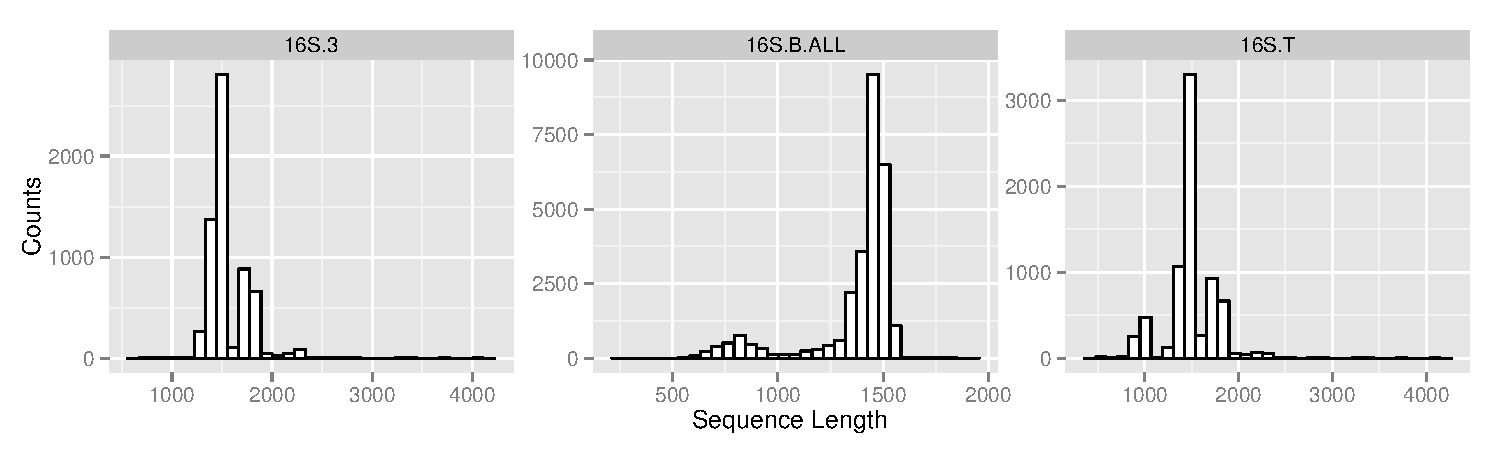
\includegraphics[width=1.0\linewidth]{{upp/length.gutell.1.30}.pdf}\\
\caption[Histogram of sequence lengths for the 16S Gutell CRW datasets.]{\label{gutell_length}  {\bf Histogram of
sequence lengths for the 16S Gutell CRW datasets.}  The histogram
of sequence lengths for the three CRW datasets demonstrates
substantial sequence length heterogeneity, especially
for 16S.T.
%a histogram of sequence lengths for 16S from the Gutell CRW datasets.  
The average length of the 16S sequence is approximately 1500.}
\end{figure}


\begin{figure}[htpb]
\centering
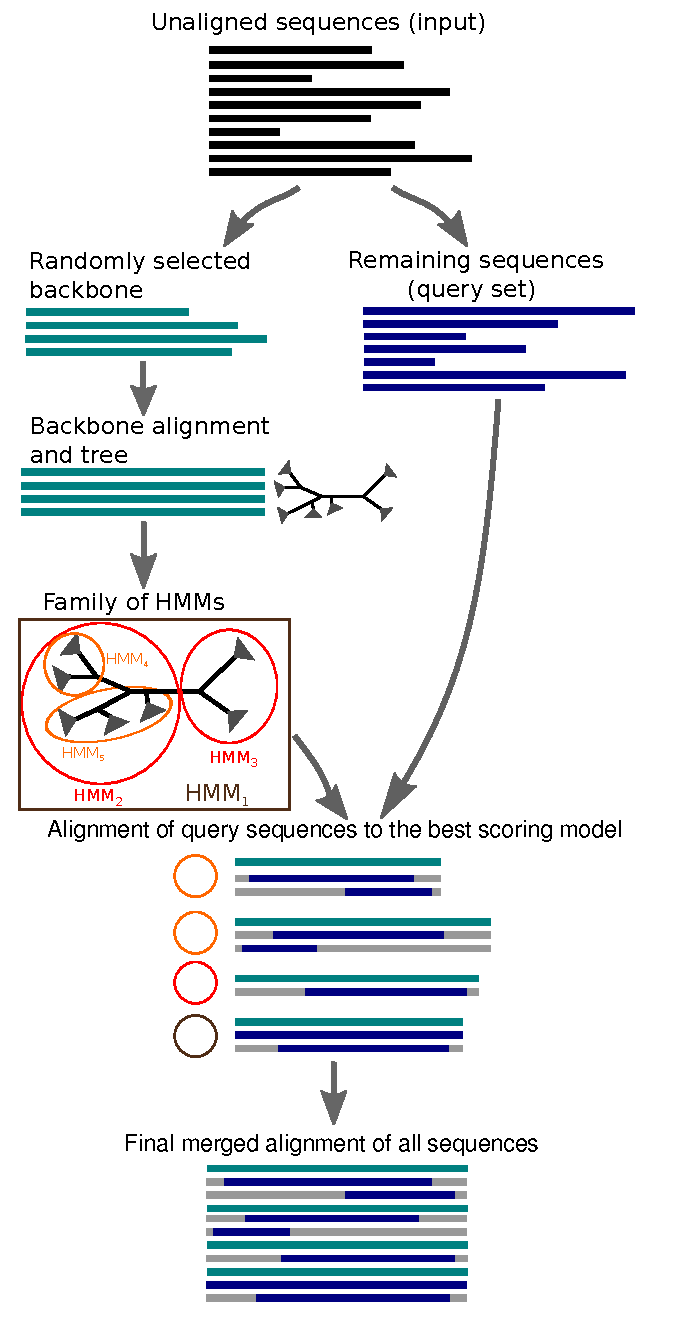
\includegraphics[width=.65\linewidth]{upp/diagram}  
\caption[Overview of the UPP algorithm.]{\label{flow_chart}  
{\bf The UPP algorithm and the HMM Family technique.}}
\end{figure}

Furthermore, many biological datasets contain
substantial numbers of 
fragmentary sequences 
(Fig.~\ref{gutell_length} and figs.~\ref{homfam_length}
and \ref{balibase_length} in the
supplementary online materials \cite{SOM}),
resulting in part from incomplete assembly or
insufficient transcript sampling.  % \cite{why-fragments}.
Although some methods (e.g., HMMER \cite{Eddy1998,HMMER} and MAFFT-Profile \cite{Katoh2012})
can add individual sequences (even short fragments) into existing alignments,
MSA methods are not designed to analyze datasets containing
a mixture of fragmentary and full-length sequences, and
have not been
tested under these conditions.
Thus, little is known about the accuracy of 
alignments on datasets of any size that contain
fragmentary sequences, nor about the accuracy of
trees estimated on such alignments.

Thus, large-scale multiple sequence alignment estimation is
a basic step in many problems, including gene tree estimation and
protein structure and function prediction, but
existing methods have not been shown to provide sufficient accuracy
on datasets that are large, that evolve under high rates of evolution,
or that contain fragmentary data. 
The new technique I present, UPP, addresses these challenges.

\section{UPP: Ultra-large alignment using Phylogeny-aware Profiles}\label{upp:algorithm}
UPP begins with unaligned sequences, and selects a subset
(called the ``backbone dataset") of the sequences,
and the remaining sequences are the ``query sequences".
 %, restricted to those that
UPP preferentially selects the backbone
sequences from  those that are considered to be ``full-length", in order to
provide robustness to fragmentary data.
UPP uses PASTA to compute an alignment and a tree on the backbone sequences
(called the ``backbone alignment" and ``backbone tree", respectively).
The backbone tree is then used to create a collection of subsets of the sequence dataset,
with subsets ranging in size from at most ten to up to the full dataset,
and all but the smallest subsets contain other subsets
(see Fig.~1, Methods, and Section \ref{upp_alg} for additional details).
UPP adds each
query sequence into the backbone alignment
using methods (HMMBUILD, HMMSEARCH,
and HMMALIGN) within the HMMER  suite of
tools, as follows. First, UPP uses HMMBUILD to build profile HMMs, one
for each subset alignment (defined to be the backbone
alignment restricted to the subset sequences); this is
called the ``HMM Family".
The fit of each query sequence
to each HMM is then assessed using HMMSEARCH; this 
returns a ``bit score", which is
a measure of the quality of the match between
the query sequence and the HMM. 
The subset HMM with the best bit score is selected, and the 
sequence is added to the subset alignment using HMMALIGN.
By transitivity, this process defines how the query sequence should
be added into the backbone
alignment. Once all the query sequences are added
into the backbone alignment, transitivity defines the final
output multiple sequence alignment. 

UPP can also be used iteratively. In the
first iteration, the UPP alignment is computed,
and a ML tree is estimated using
FastTree.
This ML tree is then used to select the backbone dataset
for the next iteration, thus ensuring
appropriate phylogenetic diversity in the backbone.
While this resampling technique is generally beneficial,
it is particularly helpful
where there is highly uneven taxon sampling (e.g., a densely sampled
in-group and very sparsely sampled distant outgroup), 
when %However, resampling is also helpful when
 fragmentary sequences are unevenly distributed throughout the
phylogeny, or when sequence lengths changed substantially
over evolutionary history.
In each of these cases, 
the technique used to select backbone sequences could
lead to backbones that fail to have
adequate representation in all the major clades -- thus reducing
the accuracy of the resultant alignment.

\paragraph{The UPP algorithm.}
I describe a single iteration of UPP run
in default mode;
see Section \ref{upp_alg} for additional details.
The input to UPP is a set of sequences.
In the first step, UPP determines whether the
dataset has fragmentary sequences, based
on the estimated median length 
of ``full-length" sequences.
Any sequence that is shorter than 75\% of this
median length,  or longer 
than 125\% of the median length, is
not considered to be full-length, and will not be 
included in the backbone dataset (except
in a ``directed sampling" step, as described
earlier).
Then, a random subset $S_0$ of 1000 full-length  sequences
is selected,
%sequences that are considered to be ``full-length"
%(defined to be with 75\% and 125\% of the known or estimated median length
%of full-length sequences for the molecule)
 and a PASTA alignment $A$ and tree $T$ are
computed on the subset.
(If the number of full-length sequences is less than 1000,
then $S_0$ is the entire set of full-length sequences.)
The set $S_0$ is called the ``backbone dataset" and
the tree and alignment computed using PASTA on 
$S_0$ are called the ``backbone alignment" and
``backbone tree".

The backbone tree is then used to produce a
collection $\mathcal C$ of subsets of the backbone
dataset, as follows.
First, $\mathcal C$ is initialized
to include $S_0$.
Then an edge in the backbone tree $T$ is found
whose removal splits the tree into two 
subtrees of approximately equal size;
this edge is called a ``centroid edge",
and the leaf sets of the two subtrees produced by removing
the centroid edge  are added to $\mathcal C$. 
At this point, $\mathcal C$ contains three sets: one
containing the entire set of backbone sequences, and two others
with roughly half the backbone sequences.
This  process is repeated on every subtree with more
than ten leaves.
Thus, the collection $\mathcal C$ contains a set of
subsets of $S_0$, where the smallest subsets might
contain fewer than ten leaves, and where every subset
(except for  the
smallest subsets) contains two other subsets.
For example, if the backbone tree contains 1000 leaves, then
$\mathcal C$ would contain one set of
$1000$ sequences, two sets of approximately $500$ sequences, four sets of
approximately $250$ sequences, etc., 
down to some number of sets
with ten or fewer sequences.

I then compute the backbone
alignment restricted to each subset of sequences in $\mathcal C$;
%omitting the sites that are fully gapped within each subset
%alignment; 
these are called the subset alignments.
I use HMMBUILD (from the HMMER3 suite of tools)
to build an HMM on each subset alignment,
with a match state for each site that has at least one
non-gap character (note that this is not the default
way of running HMMBUILD). 
This produces a set $\mathcal{H}$ of profile HMMs,
one for every subset alignment, with approximately the
same number of states in each HMM (the only
condition where different profile HMMs will have 
different numbers of states are when the subset alignments
contain different numbers of all-gap sites).

Each sequence in $S-S_0$ is called a query sequence.
I use HMMSEARCH (which takes alignment
uncertainty into account)
to compute the fit between each
query sequence and each profile HMM in $\mathcal{H}$.
%, using the local alignment command. %Nam?
%HMMER 3 is only local alignment no global alignment so not
%necessary to point this out
The HMM with the best fit (defined by the
best bit score returned by HMMSEARCH) is
selected for the query sequence.

HMMALIGN is then used to add  
query sequence $s$ to the
subset alignment $A_s$
associated to the HMM $H_s$ selected by $s$.
This produces a local alignment of $s$ to $A_s$ 
(and hence an alignment of $A_s \cup \{s\}$). 
By transitivity, 
this defines how to add $s$ into the  backbone alignment on $S_0$,
which I call the ``extended alignment for $s$".
When the sequence $s$ has 
a character  (nucleotide or amino acid)
that is not aligned to anything in the backbone
alignment, the extended alignment will have
an ``insertion site".
%that contains only one letter, contributed by query sequence $s$.


Once all the extended alignments are computed, I can merge
them all into a single multiple sequence alignment on $S$.
This approach will tend to have potentially many insertion sites,
%each produced by a single query sequence,
which  can be 
masked out during the tree estimation step to improve
speed.

UPP can be used iteratively,
but iteration only occurs if the distribution of
backbone sequences in a tree estimated on the UPP alignment
provides inadequate phylogenetic diversity.
Thus, the first step is to determine if 
all the major clades in  the estimated tree
contain at least one tenth of the
expected number of backbone sequences.
If the estimated tree passes this test, no resampling is triggered.
Otherwise, UPP uses the tree to select the backbone
sequences, ensuring that every major clade contributes
appropriately to the backbone sequence dataset.
See 
Sections \ref{commands}, \ref{hmm_commands}, and \ref{upp_alg}
for additional details.


\section{Performance evaluation}\label{upp:evaluation}
I demonstrate UPP's accuracy on a collection of biological
and simulated datasets, in comparison to leading multiple
sequence alignments. 
I compare estimated alignments 
to reference (true or curated) alignments, 
and ML trees on these alignments to 
reference trees, and record alignment error and tree error.
%Our study shows that UPP typically produces more
%accurate alignments than  the leading MSA methods for large-scale 
%multiple sequence alignment of both nucleotide and
%amino acid datasets, especially for datasets in the ``twilight zone" where
%high evolutionary distances make sequence homology 
%hard to distinguish from chance similarity.
%UPP is highly robust to fragmentary datasets,
%and fast enough to run on very large 
%datasets -- even up to one million sequences -- using 
%a small number of processors.
%Furthermore, 
%maximum likelihood (ML) trees based on UPP 
%alignments are typically 
%more accurate than ML trees based on other alignments.
%Thus, highly accurate \emph{de novo} ultra-largescale 
%multiple sequence alignment and
%tree estimation is achievable, even without supercomputers.

\paragraph{Datasets.} 
Because structural alignment and phylogenetic alignment
have different purposes and potentially different
criteria \cite{Reeck1987,goldman-benchmark}, I use both simulated and biological datasets (with structurally-based
alignments) to evaluate UPP in comparison to other MSA methods.


The simulated datasets include 1000-sequence nucleotide datasets 
with average length 1000-1023 
from \cite{Liu2009} that were
generated using ROSE \cite{ROSE}, and
used to evaluate SAT\'e in comparison
to other MSA methods on large datasets;  10,000-sequence datasets we
generated using Indelible v.~1.03 \cite{Fletcher01082009} with average
sequence length 1000;
and subsets of the million-sequence RNASim \cite{RNASim} dataset
with average sequence length 1554.5.
RNASim is a simulator for RNA sequence evolution
that I present here, 
and that was designed to simulate a complex molecular evolution process using
a non-parametric population genetic model that generates long-range statistical dependence
and heterogeneous rates.
%Tandy - write something
The simulated AA datasets include the  5000-sequence datasets 
from \cite{Price2010}, which were
generated using ROSE based
on proteins from the COG database \cite{COG},  and had
average sequence lengths
varying from 179.4 to 346.9.


The biological datasets include the three largest 
datasets from the
Comparative Ribosomal Website (CRW)  \cite{Cannone2002}, each
a set of 16S sequences. I include
the 16S.3 dataset (6,323 sequences of average length 1557,  spanning three phylogenetic domains), the 
16S.T dataset (7,350 sequences of average length 1492,  spanning three phylogenetic domains), 
and the 
16S.B.ALL dataset (27,643 sequences of average length 1371.9,  spanning the bacteria domain).  
The CRW datasets have highly reliable, curated alignments inferred 
from secondary and tertiary structures.  
I include ten 
large amino acid
datasets (10 AA) with curated multiple sequence alignments (the eight 
largest
BAliBASE datasets \cite{Thompson2011}
and IGADBL\_100 and coli\_epi\_100 from \cite{Gloor2005}); these
range in 
size from
 320 to 807 sequences and have average
sequence lengths that range from 56.7 to 886.3.
I also used 19 of the largest HomFam datasets, which are amino acid 
sequence datasets ranging in size from 
10,099 to 93,681 sequences,  and
having average sequence lengths ranging
from 29.1 to 469.8;
these datasets 
were used in \cite{Sievers2011} to evaluate protein multiple
sequence alignment methods on large datasets, and have
Homstrad \cite{homstrad} reference alignments
on very small subsets (5-20 sequences, median 7) of their sequences.
%Tandy - put in range of the reference alignment sizes

I generated fragmentary datasets by selecting 
a random subset of sequences and a random substring (of a desired
length) for each selected sequence (see 
Section \ref{frag_simulation} for full details).
Empirical statistics (number of sequences, number of sites in the reference alignment,
average and maximum p-distances, average
gap length, and percent of the matrix that is gapped) for each dataset 
and  model condition
can be found in Tables \ref{empirical_stats_simulated} and \ref{empirical_biological}.

\paragraph{Reference alignments and trees. }
For simulated datasets, the reference
alignment is the true alignment (known because
I simulate evolution and record the events); for
biological datasets, the reference alignment is the
curated structural alignment.
Reference trees for the simulated datasts are
the model trees that
generate the data.  For the biological datasets, we
use RAxML with bootstrapping on the reference alignments to
obtain ML 
trees with branch support,
and then I collapse all   branches with less than
75\% support;  this is the
same technique used in \cite{Liu2012} to
produce the reference trees on the CRW datasets.
The reference trees for the biological datasets 
are typically incompletely resolved.
In this case,  
the recovery of low support branches in the biological datasets is largely influenced by chance,  making
the FN rate preferable to the
standard bipartition error rate, also called the
Robinson-Foulds (RF) \cite{RF} error rate.
FN rates are identical to the RF
error rates when 
estimated and reference trees are fully resolved, and so
FN rates are also appropriate
for the simulated dataset analyses; 
hence, I report FN rates for all analyses, using
\cite{fasttree_tools}.

\paragraph{Fragment Simulation}\label{frag_simulation}

In order to test the robustness of different alignment methods to
fragmentary sequences, I generated datasets with both full-length and fragmentary sequences from the 1000-taxon 1000M2, 1000M3, and 1000M4 datasets, the CRW datasets, the Indelible datasets, and the RNASim 10K dataset.  For each dataset, a fraction of the sequences (12.5\%, 25\%, or 50\%) were made fragmentary by selecting a contiguous substring (length drawn from a normal distribution with mean length of 500 bps and standard deviation of 60 bps) from a random position (drawn uniformly, at random) from the original full-length sequence.  The remaining sequences that were selected to be full-length were left unmodified.

For each of the 1000-taxon fragmentary datasets, 5 replicates were generated.  For the larger CRW, Indelible, and RNASim 10K datasets, only 1 replicate was generated.
\clearpage

\paragraph{Methods. }
I use 
Clustal-Omega \cite{Sievers2011} version 2.1, 
MAFFT \cite{Katoh2005,Katoh2007} version 6.956b,
%Mafft-L-INS-i~\cite{Katoh2002,Katoh2005}, 
%Mafft-PartTree \cite{Katoh2007}, 
%MAFFT-Profile \cite{Katoh2012}, 
Muscle \cite{Edgar2004} version 3.8.31, 
Opal \cite{Wheeler2007}, %version number, Nam?
PASTA, %version number, Nam?
SAT\'e-II \cite{Liu2012}, %version number, Nam?
and UPP to compute multiple sequence alignments.
%The UPP analysis of the 16S.T dataset triggered a
%second iteration (due to uneven taxonomic distribution of fragments);
I show results for only
iteration of UPP in the main paper; see Section \ref{resample_16S}
for results using more than one iteration.
%MAFFT-Profile. 
I use FastTree \cite{Price2010} and RAxML \cite{Stamatakis2014} 
to compute maximum
likelihood trees on estimated and reference alignments.



\paragraph{Performance Metrics.}
I compare estimated alignments and their maximum
likelihood (ML) trees to reference 
alignments and trees.
I use FastSP \cite{fastsp} to 
compute
alignment error, recording
 the sum-of-pairs false 
negative (SPFN) rate (which is the percentage of the
homologous pairs in the reference alignment that
are not in the estimated alignment) and the
sum-of-pairs false positive (SPFP) rate
(which is the
percentage of homologous 
pairs in the estimated alignment that are not present in the reference alignment).
SPFN and SPFP rates are given in the SOM, and the means
of these two
alignment error rates are given in the main paper.
I report tree error using the false negative (FN) rate (also
known as the missing branch rate), which is 
the percentage of internal edges in the reference tree that 
are missing in the estimated tree.
I also report $\Delta{FN}$, the difference between 
the FN rate of the estimated tree versus the FN 
rate of the tree estimated on the true alignment, to 
evaluate the impact of alignment estimation error on
phylogenetic analysis.
Most typically, $\Delta(FN)>0$, indicating that the estimated tree
has higher error than the ML tree on the true alignment.



\paragraph{Computational resources. }
The majority of experiments were run on the
homogeneous Lonestar  cluster at
the Texas Advanced Computing Center (TACC).
Because of limitations imposed by TACC, these
analyses are limited to 24 hours, using
 12 cores with 24 GB of memory;
methods that failed to complete within 24 hours or 
terminated with an insufficient memory error message were marked as failures.  
For experiments on the million-sequence RNASim dataset,
I ran the methods on a 
dedicated machine with 250 GB of main 
memory and 12 cores and ran until an alignment 
was generated or the method failed.  
I also performed a limited number of experiments on TACC with
checkpointing, to explore performance 
when time is not limited.  


\section{Results}\label{upp:results}
\paragraph{Initial experiments. }
I let UPP(Default) denote the default version of UPP
in which I use
backbones of 1000 sequences, use PASTA to compute
the backbone alignment, and add sequences to  the backbone
alignment using
the HMM Family technique.
I also explore UPP(Fast), the variant
where I use   use backbones of 100 sequences but keep the
other algorithmic parameters fixed, and ``NoDecomp"
versions of UPP(Fast) and UPP(Default)
to indicate that
I use just one HMM instead of a family of HMMs
to represent the backbone alignment.
I show results for one iteration of UPP.


Since UPP computes its backbone using PASTA,
I compared UPP to PASTA, and included
a comparison to SAT\'e-II, focusing on
the RNASim datasets. % (Section \ref{sec:som-upp-vs-pasta}).
As shown in  \cite{PASTA},
PASTA is
more accurate than SAT\'e-II, can analyze larger datasets,
and is computationally more efficient than SAT\'e-II.
A comparison between UPP(Default), SAT\'e-II, and PASTA shows that 
UPP(Default) typically had the lowest
alignment error rates
(figs.~\ref{rnasim_pasta_alignment}-\ref{homfam_pasta_alignment})
and was much more robust to fragmentation
(fig.~\ref{frag_1000M2_pasta_alignment}). 
UPP produced more accurate trees than SAT\'e-II 
(fig.~\ref{rnasim_pasta_tree}).
PASTA had a small advantage over UPP with respect to tree estimation
on datasets without fragments
(fig.~\ref{rnasim_pasta_tree}), but was less accurate
than UPP on datasets with fragments
(fig.~\ref{frag_1000M2_pasta_tree}).
%Nam - verify that the 16S.T figure is using UPP with two iterations
UPP(Fast) was  also able to analyze larger datasets 
than PASTA and SAT\'e-II:  the  million-sequence RNASim dataset
was analyzed by UPP(Fast, NoDecomp) in 52 hours, but
PASTA failed to complete on the dataset and SAT\'e-II failed to
complete on even the 100K RNASim dataset (section \ref{early_termination}).
I focus the remainder of the discussion on Clustal-Omega, Muscle, 
MAFFT, and UPP;
results for the full set of methods can be found in Section 
\ref{sec:all_methods}.  

\subsection{Phylogenetic alignment accuracy}
I begin by evaluating UPP for phylogenetic estimation purposes.
I use simulated datasets, since these provide
true alignments and true trees, and thus allow us
to exactly quantify error in identifying true positional homology
(i.e., descent from a common ancestor \cite{Reeck1987}).

\begin{figure}[htpb]
\begin{subfigure}[htpb]{\textwidth}
  \centering
  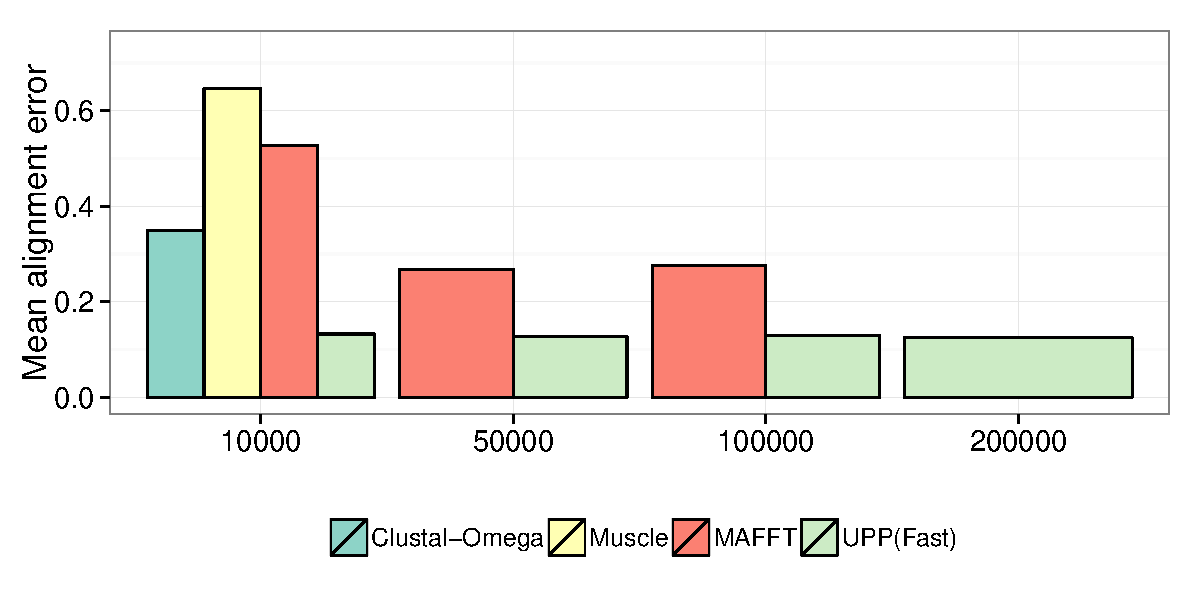
\includegraphics[width=0.60\linewidth]{{upp/rnasim.main.alignment_average}.pdf}\\
  \caption[]{Alignment error on RNASim datasets with 10K to 200K sequences}
\end{subfigure}
\begin{subfigure}[htpb]{\textwidth}
  \centering
  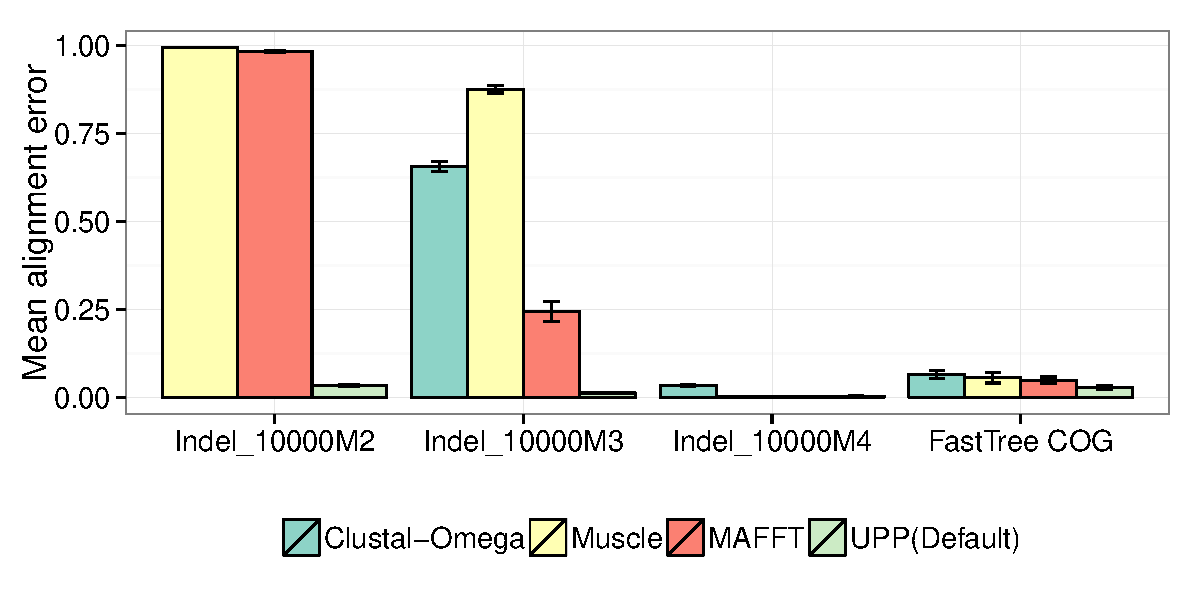
\includegraphics[width=0.60\linewidth]{{upp/all_simulated.main.alignment_average}.pdf}\\  
  \caption[]{Alignment error on other simulated datasets}
\end{subfigure}  
\begin{subfigure}[htpb]{\textwidth}
  \centering
  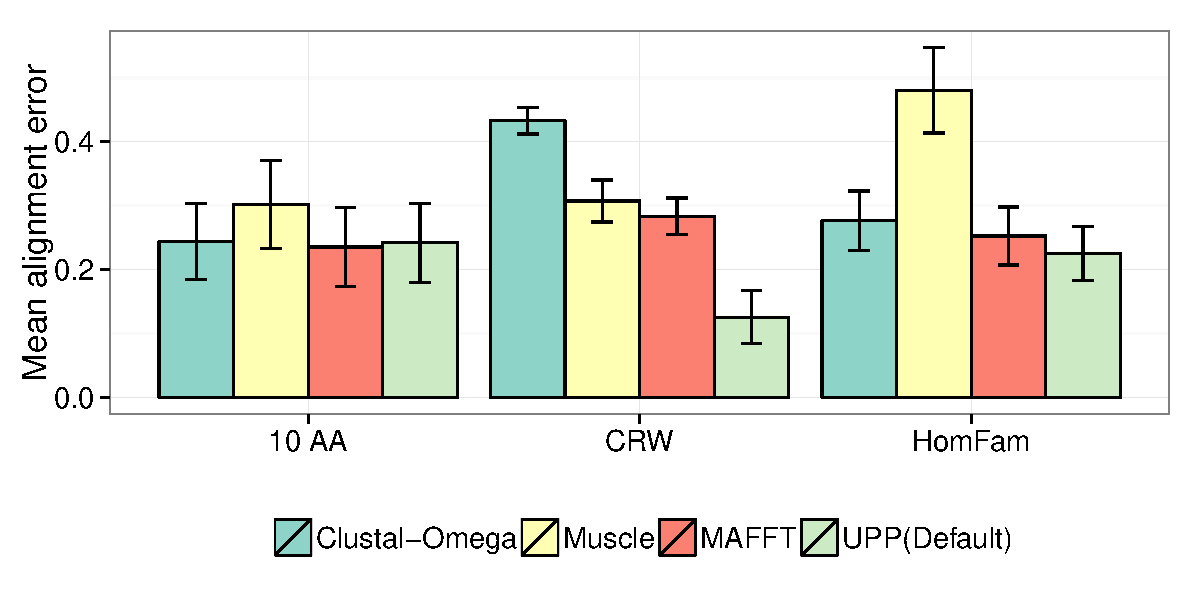
\includegraphics[width=0.60\linewidth]{{upp/all_biological.main.alignment_average}.pdf}\\  
  \caption[]{Alignment error on biological datasets}
\end{subfigure}  
\caption[Alignment error rates on different datasets.]
{\label{align_error}  {\bf Alignment error rates on 
simulated and biological datasets. }  
All methods were 
run with 24 GB of memory and 12 CPUs, and given 24 hours to complete.  
MAFFT is run using L-INS-i on the 10 large AA datasets, using default MAFFT on the FastTree COG datasets, HomFam datasets, and the CRW 16S.T and 16S.3 datasets, and using 
the PartTree command
for the CRW 16S.B.ALL dataset (default MAFFT failed to align this dataset).
Results not shown are due to methods failing to return an alignment
within the 24 hour time period on TACC, using 12 processors.
% Muscle fails to run on datasets with 50K sequences or more due to insufficient memory.  Similiarly, MAFFT-profile(Fast) fails on the 200K dataset due to insufficient memory.  Clustal-Omega fails to generate an alignment within the 24 hour time limit on datasets with 50K sequences or more.  
}  
\end{figure}


\paragraph{Alignment estimation error on RNASim datasets. }
I examined performance on the RNASim datasets with
up to 200,000 sequences, using
UPP(Fast) to
reduce running times
(results obtained using backbones of 1000
sequences showed improved accuracy but took longer; 
see Table~\ref{table:rnasim_upp_variants}).
I compare UPP(Fast) to MAFFT (default MAFFT on the 10K and 50K datasets, MAFFT-PartTree on 100K dataset),
Clustal-Omega, and Muscle (Fig.~\ref{align_error}(a)). 
Default MAFFT produced less accurate alignments %but more 
%accurate trees 
than MAFFT-PartTree on the RNASim 10K dataset (fig.~\ref{mafft_default_parttree})
and failed to complete on the 100K and larger datasets (Section
\ref{early_termination}).
%UPDATE with new results for baldr tree

UPP(Fast) succeeded in analyzing all the 
datasets within the 24 hour time limit, MAFFT-PartTree succeeded in analyzing the
datasets with up to 100K sequences, and default MAFFT successfully analyzed datasets with up to 50K sequences; however,
the other methods failed to align RNASim datasets with more than
10K sequences.
Muscle failed because it
required more than 24 GB of memory on these larger datasets, 
and Clustal-Omega 
failed to return an alignment  but
without giving an error message (see Section \ref{early_termination}
for details). % (see SOM for details).
%Nam, please check this
%This will need to be updated, looks like Mafft-PartTree might
%not have memory problem up to 100K (didn't terminate early like
%previous runs, still running.  Maybe be due to using latest version of Mafft
%Still segfaults on 200K with error message.  Will update SOM when runs complete
%/work/01722/namphuon/bin/mafft: line 2028: 10329 Segmentation fault      "$prefix/splittb fast" $legacygapopt -Z $algopt $splitopt $partorderopt $parttreeoutopt $memopt $seqtype $ model -f "-"$gop -Q $spfactor -h $aof -p $partsize -s $groupsize $treealg -i infile > pre 2>> "$progressfile"
On the RNASim 10K dataset
(Fig.~\ref{align_error}(a)), the error rates were
13.3\% for UPP(Fast),  
34.9\% for Clustal-Omega, 52.7\% for default MAFFT,
%Nam: changed MAFFT result to MAFFT-default, March 16
and 64.6\% for Muscle. 
UPP(Fast)'s 
alignment error rate was quite stable across all
numbers of sequences (up to 200,000), varying between 12.5-13.3\%.


I analyzed the million-sequence
RNASim dataset using UPP(Fast), UPP(Fast,NoDecomp),
and UPP(Default,NoDecomp),  
using  a dedicated machine, allowing the analysis to
exceed the 24 hour time limit in TACC.  
Both UPP(Fast, NoDecomp) and UPP(Default, NoDecomp) completed in less than three days 
and produced very accurate alignments %(52 versus 65 hours and 
(13.0\% and 11.1\% alignment error, respectively; see
Table \ref{alignment_large}).  
UPP(Fast) took 12 days to
align this dataset, and  produced a slightly more accurate alignment than UPP(Fast, NoDecomp) (alignment error 12.8\%).

\paragraph{Results on the Indelible NT simulated datasets. }
The 10,000-sequence Indelible simulated datasets evolved under 
low (10000M4), moderate (10000M3), or high 
(10000M2) 
rates of evolution. 
The difficulty in estimating alignments increased with the
rate of evolution; therefore,
I refer to these model conditions
as easy (10000M4), medium (10000M3), and hard (10000M2).
I ran UPP(Default), 
MAFFT-Default,
%Nam, perhaps Default MAFFT
%Still running
Muscle, and Clustal-Omega on ten replicates
for each model condition. 

UPP had very low average alignment error across 
all three model conditions:
3.3\%, 1.3\%, and 0.1\% on
the hard, medium, and easy 
% average alignment error on the hardest model condition, and 
%1.3\% and 0.1\% average alignment error on the medium and easy 
model conditions, respectively
(Fig.~\ref{align_error}(b)).
The accuracy of the other methods, however,
degraded rapidly with the increase
in the rate of evolution.   
For example, under the hard model condition,
Muscle had 99.5\% average alignment error,
MAFFT-Default had 97.9\% error 
and Clustal-Omega failed to generate an alignment
(Fig.~\ref{align_error}(b)).
Under the medium model condition,  
MAFFT-Default had 22.8\% error,  %Nam
 Clustal-Omega had 65.6\% error, %Nam?
and Muscle had 87.6\% error (Fig.~\ref{align_error}(b)). %Nam
%Nam: Numbers have all been corrected
%Nam: updated MAFFT-Default alignment March 16th
Finally, under the easy model condition,
MAFFT-Default, Muscle and UPP all had very low error (below 0.4\%),
and
Clustal-Omega had 3.4\% error (Fig.~\ref{align_error}(b) and
figs.~\ref{indelible_main_alignment} and \ref{indelible_spfn_spfp_alignment}).

\paragraph{Results on simulated AA datasets with 5000 sequences. }
%Nam - put in correct numbers - the ones that were here
%don't match the figures, so I am eyeballing them
%Nam: done
On the 5000-sequence simulated amino acid datasets,
UPP had very low error (2.9\%),
MAFFT-Default had 4.9\%, 
Muscle had 5.5\%,
and Clustal-Omega had 6.5\% (Fig.~\ref{align_error}(b),
figs.~\ref{fasttree_main_alignment_average}-\ref{fasttree_spfn_spfp_alignment}).

\paragraph{Results on 1000-sequence simulated 
nucleotide datasets. }
The nine 1000-sequence model  
conditions 
studied in \cite{Liu2009,Liu2012} varied in
gap length distribution
 and overall difficulty
(as influenced by the relative
frequency of insertions and deletions (indels) to substitutions, and rate of evolution).
Although there is sequence length heterogeneity in
these  datasets, all sequences fall within the
range considered ``full-length"; therefore, because
these datasets have only 1000 sequences,
UPP(Default) is identical to PASTA on these data.
I were able to
run    Opal and MAFFT-L-INS-i (the most accurate
version of MAFFT)
in addition to Clustal-Omega, Muscle, 
and UPP(Default).  
%see Figures
%\ref{1000_taxon_main_alignment}  and \ref{1000_taxon_main_spfn_spfp}.
Error rates varied across the model
conditions, 
but the relative performance of methods
was fairly stable:
UPP(Default) and Opal had the lowest
alignment error rates (with UPP(Default)
more accurate than Opal under 
all models except those with the lowest
rate of evolution), 
Muscle and MAFFT-L-INS-i were typically
close in error (with  about twice 
as much error as UPP(Default) and Opal),
and Clustal-Omega had the highest error
(fig.~\ref{1000_taxon_main_alignment}).
As an example, on 1000M3, one of the easiest model conditions,
UPP(Default) and Opal had
the lowest alignment errors (5.6\% and 5.4\%,
difference not statistically significant),  %Nam - please calculate
followed by MAFFT-L-INS-i (14.1\%), Muscle (15.1\%),
and finally Clustal-Omega (34.3\%).
On 1000M1, one of the hardest model conditions,
UPP(Default) had  19.9\% error, followed 
by Opal with 25.1\%, MAFFT-L-INS-i with 52.2\%,
Muscle with 52.5\%, 
and finally by Clustal-Omega with 91.8\%.
%Figure \ref{1000_taxon_main_spfn_spfp} provides results for SPFN and SPFP
%errors on these data.
%but were
%of all methods (5.6\% on 1000M3 and 19.9\% on 1000M1, the easiest and hardest model conditions, respectively) followed
%by Opal (5.4\% on 1000M3 and 25.1\% on 1000M1), with MAFFT-L-INS-i (14.1\% on 1000M3 and 52.2\% on 1000M1) and Muscle (15.1\% on 1000M3 and 52.5\% on 1000M1)
%having roughly double the alignment error, and then
%Clustal-Omega having the highest alignment error (34.3\% on 1000M3 and 91.8\% on 1000M1).

%{\bf Nam - put in numbers for the paragraph above. }
%Nam: Done

\begin{figure}[htpb]
  \centering
    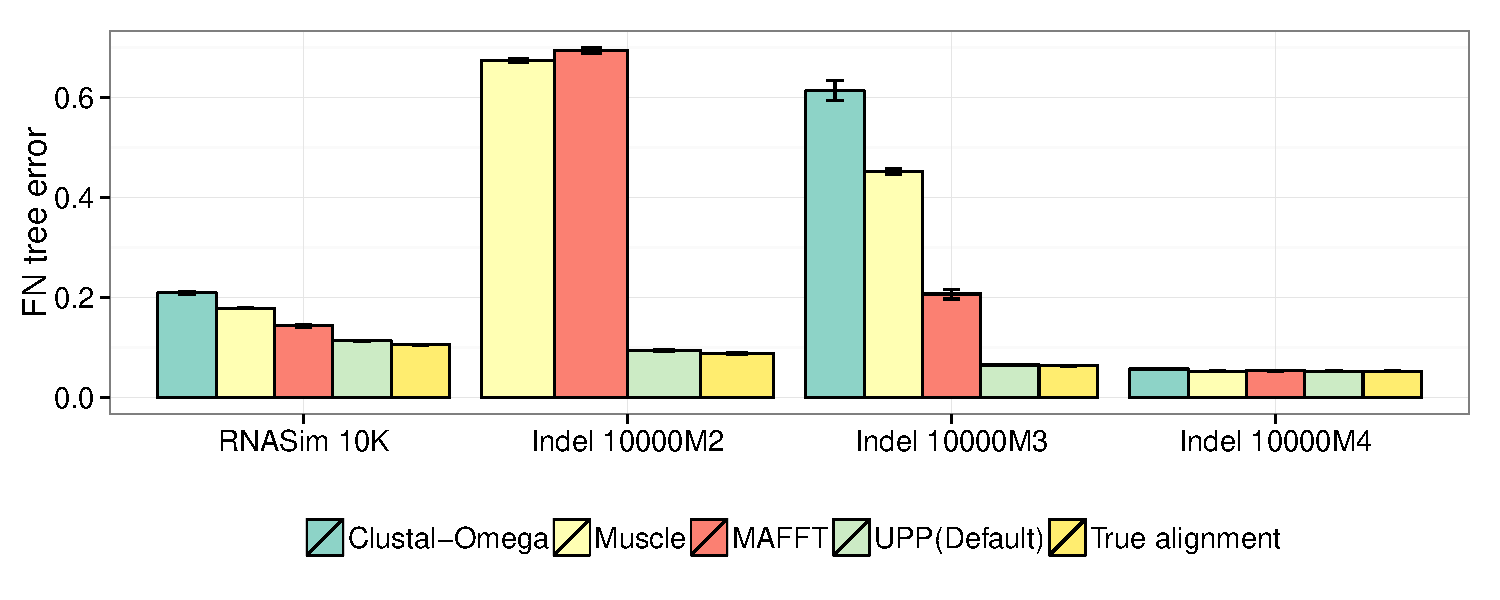
\includegraphics[width=0.9\linewidth]{{upp/large_sim.mixed.fn}.pdf}\\
\caption[Tree error on RNASim 10K and Indelible datasets]{\label{large_sim}  
{\bf Tree error on simulated datasets with 10,000 sequences.}  
I show FN tree error results on the RNASim 10K and Indelible datasets.  ML trees were estimated using FastTree under the GTR model.  All MSA methods were run with 24 GB of memory and 12 CPUs and given 24 hours to complete. MAFFT was run under the default setting on all datasets.  Standard error bars are shown.  Averages are computed over 10 replicates per dataset.  Clustal-Omega terminated with an error message on the Indelible 10000M2 datasets and thus, results are not shown.
%Muscle fails to run on datasets with 50K sequences or more due to 
%insufficient memory.  Similarly, MAFFT-profile(Fast) fails on the 200K dataset due to insufficient memory.  Clustal-Omega fails to generate an alignment within the 24 hour time limit on datasets with 50K sequences or more.  FastTree  completes within 24 hours on all tested alignments.  
}
\end{figure}

\paragraph{Impact of MSA estimation technique on phylogenetic tree estimation. }
Next, I evaluated the impact of MSA estimation on
phylogenetic tree estimation.
I show results for three of the 1000-sequence
model conditions,  each with
medium gap lengths, and varying the rate of evolution.
Under relatively low rates of evolution (1000M3), error
rates were generally low, but under moderate (1000M2) to
high (1000M1) rates of evolution, the tree error rates
increased for most methods
(fig.~\ref{1000_taxon_main_tree}).
For example, 
%UPP(Default) had the lowest tree error, with 
%$\Delta$FN ranging from 0.1-4.2\% under all nine model conditions.
on the hardest model condition (1000M1),
 the $\Delta$FN error
rates were 4.2\% for UPP(Default), 
%Nam - check this
%Done
15.4\% for MAFFT-L-INS-i, 20.5\% for Opal, 26.5\% for Muscle, and 
52.0\% for Clustal-Omega.
At the other extreme, on a very easy model condition (1000M3),
$\Delta$FN error rates were generally good:
0.2\% for UPP(Default), 
1.7\% for MAFFT-L-INS-i, 1.8\% for Opal,
and 3.7\% for Muscle; only  Clustal-Omega 
did poorly under this model condition (11.4\% $\Delta$FN).

Most methods do well  on the 5000-sequence simulated  AA datasets,
except for Opal, which failed
to align the COG438 dataset 
(terminated early due to memory error) and 
had high $\Delta$FN (12.2\%) on the other
datasets;
in comparison,
UPP(Default) had the most accurate results
(1.9\% $\Delta$FN), %Nam
followed by Muscle with 3.1\% and 
Clustal-Omega with 4.1\% %Nam?
(fig.~\ref{fasttree_main_tree}).
%Nam: Done

Performance on the Indelible and 
RNASim  datasets with 10,000 sequences (Fig.~\ref{large_sim})
show that UPP(Default)  
had very low FN error, within 0.7\%  tree error of ML on 
the true alignment, even on the hardest Indelible datasets.  
With the exception of the easiest Indelible model conditions
where all methods perform equally well (within 0.4\% tree error of ML on tree alignment), 
the other methods produced significantly less accurate trees.  
For example, on the Indelible 10000M2 model, 
UPP had 0.6\% $\Delta$FN error,
 MAFFT had 58.1\%, Muscle had 58.6\%,  and 
Clustal-Omega failed to generate an alignment 
(Fig.~\ref{large_sim} and section \ref{early_termination}).  
%Nam: updated MAFFT-Default tree error March 16th
  
I computed ML trees using
FastTree on three UPP alignments 
(UPP(Fast), UPP(Fast,NoDecomp), and  
UPP(Default,NoDecomp))
of the million-sequence RNASim dataset.
Despite the large number of 
sequences and relatively few sites (1500 average
sequence length), 
FN tree error was 
still very low: 8.4\% for UPP(Fast,NoDecomp),
 7.7\% for UPP(Default,NoDecomp),   and 7.5\% for UPP(Fast),
so that $\Delta$FN was between
2.0-2.8\% for all UPP variants I tested.
%(Figure \ref{fig:million}).  %fast with decomposition), with UPP(Fast) resulting in the lowest tree error.  
The phylogenetic accuracy  of these
trees is noteworthy, given that the  % both UPP(Fast) and
true alignment; see Table~\ref{alignment_large}) given
sequences were not particularly long  (1500 sites, on average),
indicating not only the quality of the
sequence alignment produced by UPP(Fast) and UPP(Fast,NoDecomop), but
FastTree's ability to produce reasonable results on
extremely large datasets.
%Tandy, Nam, Siavash - note this is not GTR evolution
%Nam, fill in value for UPP(Default,no-decomp) when available (March 6)
%Results on other datasets show
%similar trends (see SOM~\ref{upp_variant}). %Tandy - give location
%Nam:  Add in this section, currently only have UPP variants on RNASim
%New results for new backbone protocol on Gutell not done yet


I used the RNASim datasets to explore the 
impact of increased taxon sampling, which  is expected to improve
phylogenetic accuracy \cite{zwickl_increased_2002}.
As expected, tree error was reduced with increased
taxon sampling when using 
true alignments:
ML trees had  
FN error rates of
10.6\%, 8.1\%, 6.9\%, and 6.1\% on the RNASim 10K, 50K, 100K, and 200K datasets, 
respectively. % (Table \ref{table:XXX}).
I then tested this on the UPP alignments, to see if the
 beneficial impact
held for alignments estimated using UPP.
Maximum likelihood trees computed on 
UPP(Fast) alignments also reduced in error 
with increasing numbers of taxa:
UPP(Fast) trees had 11.8\% FN error
at 10K sequences, 9.4\% at 50K
sequences, 8.3\% at 100K sequences, 7.6\% at 200K sequences, and
7.5\% at 1,000,000 sequences.
%Nam - need to know where the results on the true alignment are
%provided - and also for the million sequence dataset
%perhaps add them to Table 1?
Thus, UPP alignments are good enough to show the beneficial
impact of increased taxon sampling on phylogenetic accuracy (similar
patterns hold for other UPP variants, see Table \ref{table:rnasim_upp_variants}).
%Nam, add something for UPP(Fast,NoDecomp), UPP(Default,NoDecomp), etc?
% \cite{zwickl_increased_2002}. 


\subsection{Structural alignment accuracy}

I used biological datasets with structurally-defined reference
alignments to evaluate UPP with respect to structural alignment
accuracy.
On the ten amino-acid datasets (10 AA) with
full alignments, 
Muscle had the highest average alignment error (30.2\%)
and the other methods (MAFFT-L-INS-i, Opal, 
and UPP) have very close
error rates between 23.5\% and 24.3\% (Fig.~\ref{align_error}(c),
figs.~\ref{balibase_main_alignment_mean}
and \ref{balibase_main_alignment_sop}).  
 % and \ref{balibase_main_tree} for full results.
The 19 HomFam datasets and three CRW datasts are too
large for MAFFT-L-INS-i or Opal, and so I use
MAFFT-Default (or MAFFT-PartTree on CRW 16S.B.ALL) on these data.
On the 19 HomFam datasets, 
Muscle failed to align
two datasets, and had generally very
high error on those it could align;
the other methods succeeded in 
aligning all the datasets. 
Comparing methods on just the 17 datasets 
that Muscle succeeded in aligning, 
UPP had 22.5\% alignment error, followed by
MAFFT-Default with 25.3\% error, 
Clustal-Omega with 27.7\% error, %Nam???
%Nam: Updated with Mafft-Default resutls
and Muscle with
48.1\% average error
%Nam: corrected
(Fig.~\ref{align_error}(c),
see also figs.~\ref{homfam_main_alignment} and \ref{homfam_main_spfn_spfp}
for additional results). 
%Nam, did you try to run MAFFT-default on HomFam?
%Yes, results are now in
MAFFT-default failed to run
on the 16S.B.ALL CRW dataset
(see Section \ref{early_termination}),
and so I used MAFFT-PartTree for that dataset; however,
I report
MAFFT-default for 16S.3 and 16S.T.
UPP   had the lowest average alignment error across
these three datasets (16.3\%), 
MAFFT had 28.8\%, 
Muscle had 30.7\%, and
Clustal-Omega  had 43.3\% (Fig.~\ref{align_error}(c)).
% was run using default setting for 16S.3 (25.2\% alignment
%error) and 16S.T (30.4\% alignment error),
%but could not be run in that setting on the
%16S.B.ALL dataset; hence, I report 
%MAFFT-PartTree (29.4\% alignment error).
%Note:  Mafft-Default does better on 16S.T, may be better than PartTree on CRW
% currently running it on 16S.B.ALL so once that's done numbers may change
Overall, UPP had the the best or close to the best results 
on these biological datasets, showing 
that UPP produced excellent alignments  
according to structural benchmarks on both nucleotides and amino acid sequences.
%gives good results on both nucleotide and amino acid datasets.
%However, Clustal-Omega did better on
%amino acid datasets than on nucleotide datasets, and
%Muscle did better on nucleotide datasets than on amino acid datasets.
%Nam, Siavash,  and Tandy - put this into the discussion 

\begin{figure}[htpb]
\begin{subfigure}[htpb]{\textwidth}
  \centering
  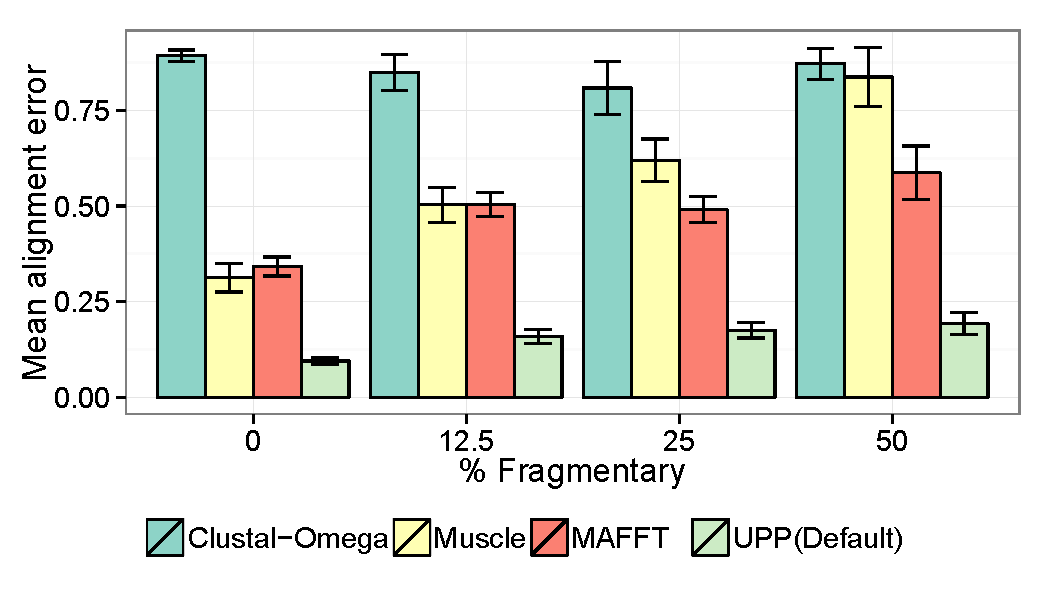
\includegraphics[width=0.85\linewidth]{{upp/frag.1000M2.alignment_average.main.500}.pdf}\\  
  \caption[]{Fragmentary 1000M2 model conditions}
\end{subfigure}
\begin{subfigure}[htpb]{\textwidth}
  \centering
  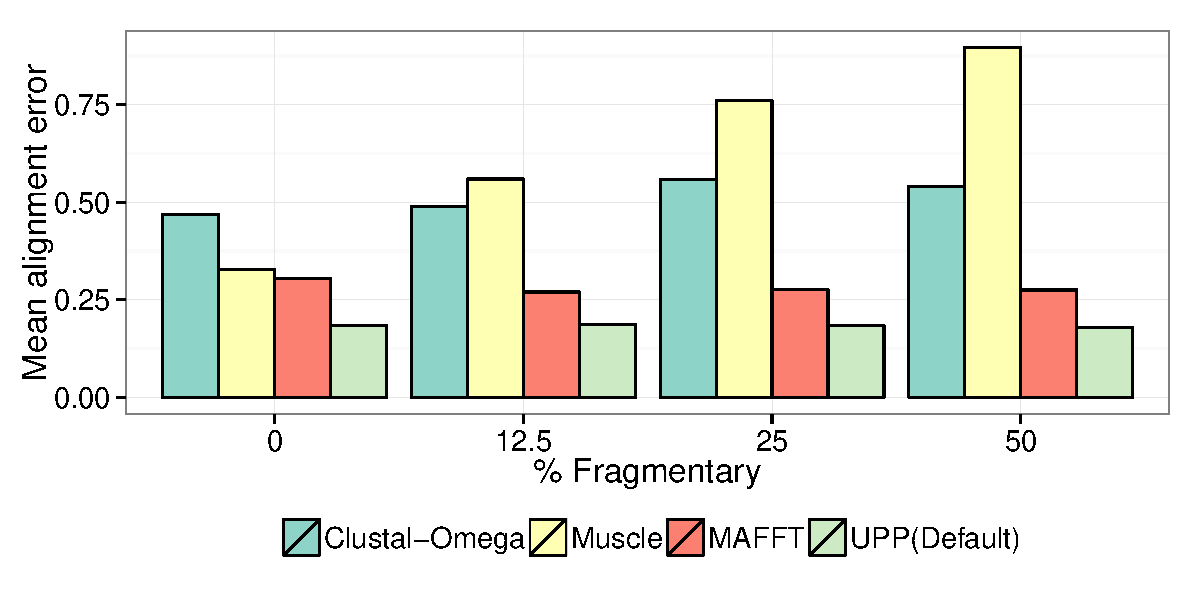
\includegraphics[width=0.85\linewidth]{{upp/frag.16S.T.alignment_average.main.500}.pdf}\\  
  \caption[]{Fragmentary CRW 16S.T datasets}
\end{subfigure}
\caption[Impact of fragmentary sequences on alignment error.]{\label{fig:fragmentary}  
{\bf Impact of fragmentary sequences on alignment error. }
I show alignment error rates for different methods on 
the 1000-sequence 1000M2 datasets and the 7350-sequence CRW 16S.T  
dataset, but include results where a
percentage of the sequences are made fragmentary, varying
the percentage from 12.5\% to to 50\%.
Fragmentary sequences have average 
length 500 
(i.e., approximately half the average sequence length for 1000M2,
and approximately one third the average sequence length for 16S.T).  
MAFFT is run using L-INS-i on the 1000M2 datasets and
using MAFFT-Default on the 16S.T datasets. 
} 
\end{figure}
\subsection{Results on fragmentary datasets. }
Figure \ref{fig:fragmentary} shows alignment
error on fragmentary
versions of the 1000M2 simulated datasets and the
CRW 16S.T biological dataset, varying
the percentage of fragmentary sequences from 0\% to 50\%, with
average fragment length 500 (roughly half the length of the full-length 1000M2 sequences and one third the length of the full-length 16S sequence). 
UPP(Default) had substantially lower error than the other
methods, at all levels of fragmentation for both datasets.
In most cases, alignment
error  increased  as the amount of fragmentary data
increases, but methods differed in their responses.
Muscle was the most impacted by 
the amount of
fragmentary data, with
very large increases in alignment error
as the amount of fragmentary data increases.
MAFFT-default
was  also impacted, but not as
severely as Muscle.
UPP and 
Clustal-Omega were largely unaffected by
fragmentation on these data (with error rates
that change only in small ways); however,
Clustal-Omega had poor accuracy consistently,
while UPP had consistently good accuracy.
Interestingly, the relative performance
of methods changed with the amount of
fragmentation; for example, 
Muscle was more accurate than 
Clustal-Omega on the
16S.T dataset before I introduce fragmentation,
but less accurate when 12.5\% of the
sequences were fragmentary (Fig.~\ref{fig:fragmentary}(b)).
Differences between methods were reduced on
model conditions with lower rates of evolution, but
UPP(Default) still demonstrated greater robustness to 
fragmentary data than the other methods (SOM~\ref{sec:all_frag_methods}).

Phylogenetic accuracy was also impacted by 
fragmentary data, but responses varied by the alignment method.
Results on the RNASim 10K datasets (Fig.~\ref{tree-frag})
with fragmentation varying from 0\% to 50\%, and
all fragments of length 500 (i.e., about one third of
the average length of the full-length sequences)
show that UPP(Default) and MAFFT-default were both
highly robust to fragmentary data ($\Delta$FN error rates 
only changing by 3\% for UPP and 2\% for MAFFT-default).
In contrast,  tree errors for Clustal-Omega and Muscle were very 
impacted by fragmentation.
Muscle had 7.3\% $\Delta$FN on full-length sequences,
and then 35.6-49.0\% $\Delta$FN under all the fragmentary
conditions.
Clustal had 9.1\% $\Delta$FN on full-length sequences,
and then 25.4\%-25.8\% on the fragmentary conditions.
Furthermore, while both UPP(Default) and MAFFT-default
were highly robust to fragmentary data, UPP(Default) had better
accuracy under all levels of fragmentation on
this model condition: 0.8\% $\Delta$FN on
full-length sequences, and at most 3.9\% $\Delta$FN
even when half the sequences are fragmentary.
MAFFT-default had 5.9\% $\Delta$FN for full-length
sequences, and $\Delta$FN between 5.8\% and 7.1\%
on the fragmentary sequences.

\begin{figure}[htpb]
  \centering
  %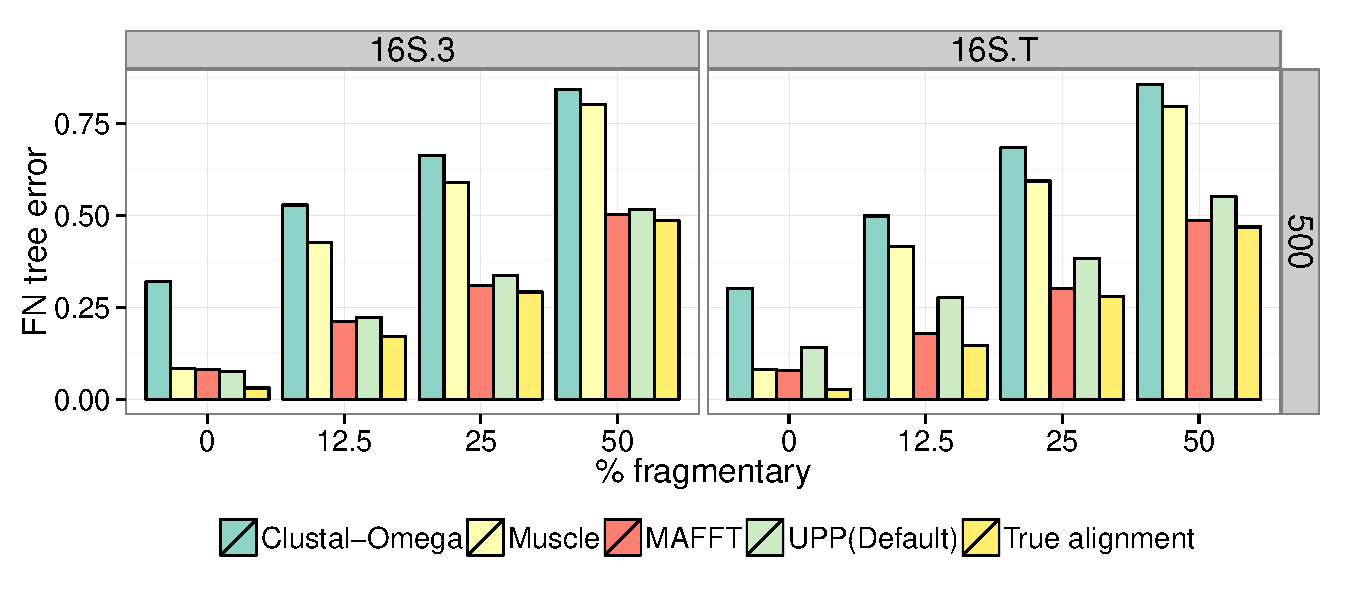
\includegraphics[width=0.90\linewidth]{{upp/large_fragmentary.gutell.fn.main}.pdf}\\
  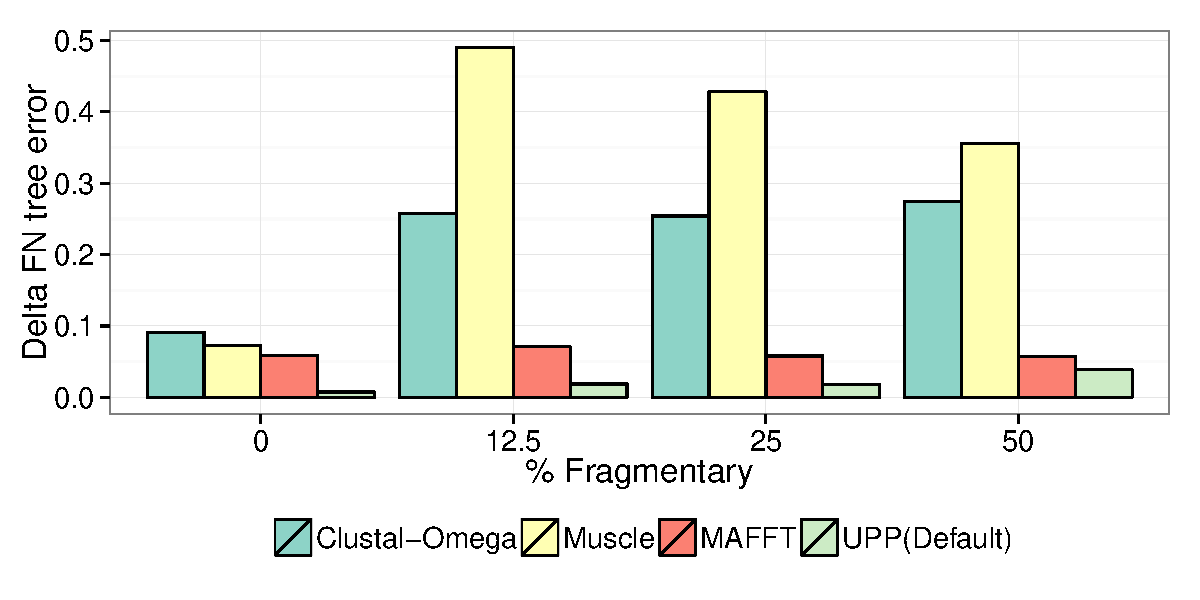
\includegraphics[width=0.90\linewidth]{{upp/frag.10000.delta_fn.main.500}.pdf}\\
  \caption[Tree error on fragmentary RNASim 10K datasets]
{\label{tree-frag}
{\bf Impact of fragmentation on tree error for the RNASim 10K datasets. }
I show the $\Delta$FN  error rates of
maximum likelihood  trees computed using FastTree under
the GTR model on
alignments computed using Clustal-Omega, Muscle,
MAFFT-Default, and UPP(Default), on the
RNASim 10K dataset, including results on versions of the
dataset where I make some of the sequences fragmentary.
All fragments have average length 500, but I vary the percentage of the
dataset that is fragmentary.
%Nam - would be better if I had RAxML, but I guess
%that will have to wait.
%Also, are these MAFFT-PartTree or MAFFT-Default?
}
%Nam - would be better to show Delta-FN.
%might also be good to include results on full-length sequences.
%also, order them in terms of increasing levels of fragmentation,
%just like you did for the alignment error.
%I will fix this
\end{figure}



Figure \ref{fragmentary_1000_taxa_tree} shows
similar trends for the 
fragmentary 1000M2
and 1000M3 datasets.
% but MAFFT (run using the most
%accurate setting, L-INS-i) is not as robust to fragmentation.
$\Delta$FN on the fragmentary 1000M2 datasets
ranged for UPP(Default) from 2.5-4.7\%,
from 34.7-65.0\% for Muscle,
and from 55.8-70.8\% for Clustal-Omega (fig.~\ref{fragmentary_1000_taxa_tree}).
Results on fragmentary versions of the 1000M3 model 
condition, which has a lower rate of
evolution than 1000M2, show $\Delta$FN for UPP(Default)
ranging from 0.2-2.2\%,
while $\Delta$FN ranged from 12.7-27.8\% for
Muscle and from 18.8-57.2\% for Clustal-Omega.
MAFFT-L-INS-i showed somewhat
better tolerance to fragmentary
data than Clustal-Omega or Muscle, but still
had high $\Delta$FN rates: 18.1-43.5\% error on the 1000M2 model condition, and 4.0-14.1\% for 1000M3.

\subsection{Factors influencing accuracy}
%Using the HMM Family technique instead of a single HMM
%produced a large impact on tree estimation error (Table 1
%and figs.~\ref{rnasim_upp_tree} and ~\ref{gutell_upp_tree}), but
%had a smaller impact on alignment error (figs.~\ref{rnasim_upp_alignment} and ~\ref{gutell_upp_alignment}).
The choice of alignment method
to compute the backbone alignment has an impact on final alignment and
tree accuracy:
comparing PASTA, MAFFT-L-INS-i, Muscle, and Clustal-Omega
for backbone alignment estimation, I found that
PASTA and Muscle backbones yielded the best alignment accuracy
(fig.~\ref{rnasim_alignment_alignment}) 
but PASTA and MAFFT-L-INS-i backbones yielded the best tree accuracy
(fig.~\ref{rnasim_alignment_tree}).
The choice of technique used to align query sequences
to the backbone alignment also impacts alignment and tree error
(Table 1 and figs.~\ref{rnasim_backbone}, \ref{rnasim_upp_tree}, \ref{gutell_upp_tree},
\ref{rnasim_upp_alignment}, and \ref{gutell_upp_alignment}), with the HMM Family technique giving
the best results compared to a single HMM or MAFFT-Profile with
either -{}-add or -{}-addfragments.

I found that the error of 
the backbone alignment and the 
alignment generated by three different ways of running UPP 
(default setting, and aligning query sequences using MAFFT-Profile)
were strongly correlated
(Fig.~\ref{backbone_error},
Pearson’s correlation coefficient 0.897; p-value=2.29e-10). 
Furthermore,
alignment errors for UPP(Default)  were
very close to the backbone alignment error, with root mean square difference (RMSE)
of 0.020, and 
closer to the backbone alignment error than those
produced by UPP using MAFFT-profile 
(RMSE of 0.024 for MAFFT-profile-{}-addfragment
and 0.051 for MAFFT-profile-{}-add, fig.~\ref{backbone_error}).
%in alignment error of 0.020 for UPP versus 0.024 and 0.051 for MAFFT-profile “addfragments”
%and MAFFT-profile “add”).
Thus, while the three versions of UPP all showed
good correlations between backbone alignment error and 
final alignment error, 
the use of the HMM Family
technique gave the best correlation, and helps
UPP to scale alignment accuracy obtained on
small subsets to large datasets.







\subsection{Running time. }
%Nam - can you give running times (approximately) on other datasets, not just RNASim?
%Nam: I can get numbers for Gutell, remove this note once done

\begin{figure}[htpb]
%\begin{subfigure}[htpb]{\textwidth}
  \centering
  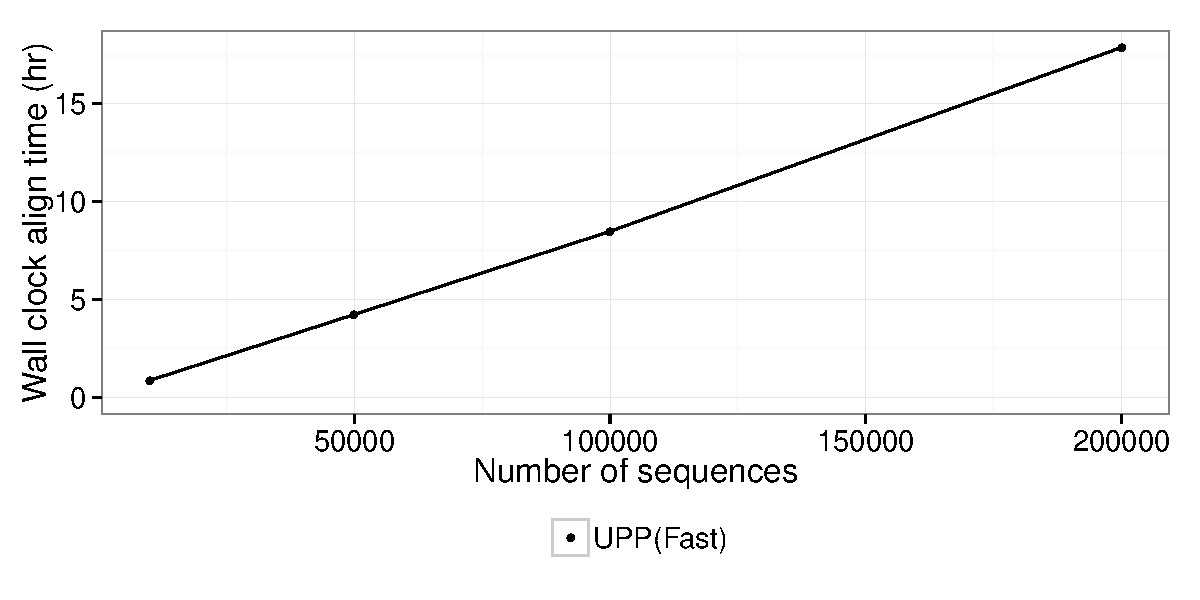
\includegraphics[width=0.95\linewidth]{{upp/rnasim.only_upp.wall_align_time}.pdf}\\
 % \caption[]{Wall clock alignment time (hr)}
%\end{subfigure}
\caption[Running time for UPP(Fast) on the RNASim  datasets.]
{\label{running-time}  {\bf Running time for UPP(Fast) on the RNASim
datasets. }
I show running time for UPP(Fast) on RNASim datasets
with 10K, 50K, 100K, and 200K sequences.
UPP(Fast) uses a backbone of size 100, computes the backbone
alignment using PASTA, and then aligns the remaining sequences
using the HMM Family technique.
All analyses were run on TACC with 24 GB of memory and 12 CPUs.
%MAFFT is run using the PartTree command on all these datasets.
%Results not shown are due to methods failing to return an alignment
%within the 24 hour time period on TACC, using 12 processors.
% Muscle fails to run on datasets with 50K sequences or more due to insufficient memory.  Similiarly, MAFFT-profile(Fast) fails on the 200K dataset due to insufficient memory.  Clustal-Omega fails to generate an alignment within the 24 hour time limit on datasets with 50K sequences or more.  
}
\end{figure}
%Nam - remove "Method"
%Nam: done


\begin{table}[htpb]
\caption[UPP variants on the RNASim datasets.]{\label{table:rnasim_upp_variants}
{\bf Results for UPP variants on the RNASim datasets.}
I show results for different
variants of UPP on the RNASim datasets with 10,000 to 200,000
sequences. 
I report the average alignment error, 
$\Delta$FN error (the difference
between the error on the true alignment
and on the estimated alignment), 
and running time (in CPU hours), using
12 processors with 24Gb of memory.
The default setting for UPP is denoted
Default; it uses a backbone of size 1000, uses PASTA 
to compute the backbone alignment, and the HMM Family technique;
Fast is obtained by using backbones of size 100 and keeping
all other settings constant.
The ``ND'' versions of these two methods replace the HMM Family
technique with a single HMM.
Default-MP uses MAFFT-Profile (with -{}-add, denoted ``A'',
or with -{}-addfragments, denoted ``AF'') to add the query sequences into the
backbone alignment, and otherwise is identical to Default;
Fast-MP differs from this only by using
a backbone of size 100.
}
\centering
\scalebox{0.90}{
\begin{tabular}{|l|l|r|r|r|r|}
\hline
Number seq. &Method&Align.~error&FN&$\Delta{FN}$&Time (hrs)\\
\hline
10,000&Fast-ND&13.1\%&14.2\%&3.6\%&0.1\\
10,000&Default-ND&11.2\%&13.6\%&3.0\%&0.2\\
10,000&Fast&13.3\%&11.8\%&1.2\%&0.9\\
10,000&Default&10.3\%&11.4\%&0.8\%&6.7\\
10,000&Fast-MP-A&26.2\%&18.0\%&7.4\%&0.2\\
10,000&Default-MP-A&14.0\%&14.8\%&4.2\%&0.3\\
10,000&Fast-MP-AF&17.8\%&15.5\%&4.9\%&1.0\\
10,000&Default-MP-AF&12.7\%&12.3\%&1.7\%&6.5\\
\hline
50,000&Fast-ND&12.2\%&10.7\%&2.6\%&0.4\\
50,000&Default-ND&12.0\%&10.5\%&2.5\%&0.9\\
50,000&Fast&12.7\%&9.4\%&1.3\%&4.2\\
50,000&Default&11.2\%&8.6\%&0.5\%&44.0\\
50,000&Fast-MP-A&33.6\%&13.8\%&5.7\%&2.1\\
50,000&Default-MP-A&16.0\%&10.1\%&0.2\%&3.5\\
\hline
100,000&Fast-ND&13.5\%&9.9\%&3.3\%&0.8\\
100,000&Default-ND&11.2\%&9.4\%&2.8\%&1.9\\
100,000&Fast&13.0\%&8.3\%&1.4\%&8.5\\
100,000&Default&11.1\%&7.6\%&0.7\%&82.3\\
100,000&Fast-MP-A&40.2\%&10.2\%&3.3\%&10.7\\
\hline
200,000&Fast-ND&12.4\%&8.5\%&2.4\%&1.9\\
200,000&Default-ND&11.3\%&8.6\%&2.4\%&6.1\\
200,000&Fast&12.5\%&7.6\%&1.4\%&17.9\\
200,000&Default&10.6\%&6.8\%&0.7\%&151.1\\
\hline
\end{tabular}}
\end{table}

Running times for UPP(Fast) on the RNASim datsets
with up to 200,000 sequences, using 12 processors,
show a close to linear trend, so that
UPP(Fast) completes on 10K sequences in 55 minutes, 
on 50K sequences in 4.2 hours,
on 100K sequences in about 8.5 hours,
and on 200K sequences in about 17.8 hours (Fig.~\ref{running-time}).
Table \ref{table:rnasim_upp_variants} explores
the trade-off between running time and 
accuracy (both alignment and tree)  of 
UPP variants.
For example,  using UPP(Fast) instead of UPP(Default)
reduces the running time substantially (by a factor
of 7 to 10) and produces only a small
increase in tree error and 
alignment error.
However, UPP is extremely parallelizable, and so
speed-ups are easily achieved through increasing
the number of processors.

\section{Conclusion and future work}\label{upp:conclusion}
Although the relative  performance
of multiple sequence alignments 
varied by datasets,   UPP in most cases showed improved alignment accuracy compared
to PASTA, SAT\'e-II, Clustal-Omega, Muscle, 
and MAFFT. 
By design, 
UPP(Default) is identical to PASTA on datasets without fragments and at most 
1000 sequences, but UPP is highly robust to fragmentary data whereas PASTA is not. 
On larger datasets,
UPP alignments tend to be more accurate than PASTA alignments, 
but ML trees based on PASTA alignments (for fragment-free datasets) are typically
more accurate than ML trees based on UPP alignments. 
However, on large datasets, 
ML trees estimated on UPP alignments are typically more accurate than 
ML trees based on all other methods (including SAT\'e-II). 
Moreover, for datasets with fragmentary sequences,
UPP provided the best alignment and tree accuracy of all the methods I tested.
Finally, UPP was the only method I tested that was able to analyze the million sequence RNASim dataset. 

UPP exhibits great scalability, both with respect to
running time (which scales in a nearly linear manner)
and parallelism, but also with respect to alignment accuracy.
For example, my study showed the alignment error on the backbone alignment is quite close to the alignment error on the alignment
returned by UPP(Default) (Section~\ref{backbone_alignment_error}), 
and this close relationship between the accuracy of the backbone alignment
and the final alignment is weaker when I use MAFFT-Profile
second iteration) and I didn't fully explore using a single HMM other than RNASim
instead of an HMM Family to align query sequences. 
Thus, the HMM Family technique is a key algorithmic 
technique to providing scalability for alignment accuracy, so that
large datasets can be aligned nearly as accurately as smaller datasets.  

However, the other algorithmic techniques also contribute to 
UPP's improved accuracy.
Restricting the backbone to full-length sequences improves
the robustness to fragmentary sequences, and
the re-sampling technique improves the close relationship between the
backbone alignment accuracy and the final alignment accuracy.
Using PASTA for the backbone alignment gives better results
than using less accurate alignment methods, 
and because PASTA is computationally efficient it also
makes it feasible to use large backbones.
Thus, the different algorithmic steps work together to
provide the improved accuracy, scalability, and robustness
to fragmentary sequences.
Furthermore, while good accuracy with respect to
structural benchmarks
was achieved using simpler versions of UPP (e.g.,
using MAFFT-L-INS-i instead of PASTA for the backbone alignment,
or using a single HMM rather than the HMM Family Technique to
align query sequences), 
the best accuracy was
obtained using my default setting, 
which also gave better results on the phylogenetic benchmarks.
Thus, UPP has excellent accuracy with respect to 
both phylogenetic and structural benchmarks, indicating
that alignments produced by UPP are highly accurate 
with respect to  positional homology and also structural homology (see
\cite{Reeck1987} for further discussion of these 
related but different concepts).

By design,
UPP is a highly modular algorithm, 
and substitutions in its algorithmic steps could lead to additional
improvements.  Because my results show that  
using small backbones
reduces accuracy only slightly, this opens the possibility of 
using sophisticated but computationally intensive
multiple sequence
alignment methods (for example, 
statistical methods based on stochastic models of sequence evolution involving
indels \cite{rs06,jordan-pnas2013}) 
to produce the backbone alignment.
The HMM Family technique is another part of
this pipeline that could be improved, for example
through using new techniques to compute HMMs (which might incorporate
structural information) or to add query 
sequences to alignments (another active area of research).  
Thus, UPP is an algorithmic paradigm rather than a specific
method, and future work will explore the design space enabled by
this paradigm.

In summary,  UPP enables highly accurate analyses of
sequence datasets that have been considered too difficult
to align, including
datasets that evolved with high
rates of evolution,   that
contain fragmentary sequences, or that are very large. 
While datasets
like these are increasingly being generated in large-scale
sequencing projects, 
the limited ability to analyze these datasets has discouraged
biologists from using the full range of their data. 
Instead, large-scale transcriptomic
and genomics projects often sub-sample from the available data
(in terms of taxa, genomic regions, and sites within genes)
in order to obtain datasets that are small enough, 
that evolve sufficiently slowly, and that do
not contain fragmentary data, so that 
available MSA methods can be reliably run on these datasets.
% Tandy, Nam, see if you agree with this addition.
% (I don't feel strongly about including this at all) 
%Therefore, UPP's increased MSA accuracy
%even on large datasets with high evolutionary rates
%enables the use of more data 
%in downstream analyses such as phylogenetic reconstruction.
%however, whether including more data 
%improves those downstream analyses
%likely depends on the application,
%and requires careful study. 
%Siavash - I took it out because the main point is in the next paragraph

UPP's robustness to fragmentary data, and its high
accuracy even for ultra-large datasets with
high rates of evolution,  
increases the range of genomic data that can be 
used in scientific studies.
As a result, scientific questions that would be improved through 
larger sequence datasets
might be able to be addressed with greater accuracy
using UPP. A prime case of where UPP could be useful is
for phylogeny estimation of
rapid radiations or deep evolution, since phylogeny estimation
 is often improved by
dense taxon sampling \cite{zwickl_increased_2002}. 
For example, the avian genome project is planning to 
eventually sequence all roughly 10,000 living bird species,
and such efforts require scalable and accurate alignment 
techniques such as UPP. % and PASTA?
However, datasets
on  smaller numbers of taxa can also
%be extremely large for multi-copy genes, 
include extremely large multi-copy gene families
(e.g., the 1KP  gene sequence datasets for 
1000 species and more than 100,000 sequences). 
Understanding the evolutionary history of these large gene families
requires gene family trees  and alignments, 
that can easily involve many tens of thousands of
sequences.
Thus, UPP is a tool for both current and future genomics and
transcriptomics projects, that will  enable
biologists to utilize the full range of their data to 
address biological problems of broad interest.


% \subsection{Comparison to previous work. }
% MSA estimation for the purpose of structure and function
% prediction
% of protein sequences (and in some cases of RNA sequences)
% is often based on machine learning models such as
% templates or profile Hidden Markov
% Models (HMMs) \cite{Eddy1998}.
% These models are used  to represent a
% seed alignment (typically
% a curated structural alignment) for the
% molecule, which is then coupled with
% methods, such as HMMALIGN \cite{HMMER} and
% MAFFT-Profile \cite{Katoh2012}, to add the
% input sequences
% into the seed  alignment and  produce
% a final multiple sequence alignment.
% Similarly, profile HMMs for different protein
% families and superfamilies are provided in
% databases such as Pfam \cite{Punta2012} and
% PhyloFacts \cite{Krishnamurthy2006},  and
% can be used to
% build multiple sequence alignments.
% However,   these ``template-based" methods
% (e.g., \cite{neuwald2009,Nawrocki2009,ShangGardnerGutell})
% can only be used to align
% sequences that match the seed alignment, and so are not
% \emph{de novo} MSA methods.
% PROMALS \cite{promals}, SATCHMO \cite{satchmo03}, and SATCHMO-JS \cite{kimmen2010}
% are protein MSA methods that build HMMs during
% the course of the alignment estimation, and
% so can be used in \emph{de novo}
% alignment; unfortunately, these methods
% %these methods
% are computationally intensive because they
% perform a sequence of HMM-HMM alignments
% to construct their final alignment, and so
% cannot be used on large datasets.


% Phylogenetic placement is a related problem
% where profile HMMs have also been used:
 % the input is
% a set of query sequences and a reference
% tree and alignment, and the objective is
% to find an edge in the reference tree
% for each query sequence.   
% SEPP \cite{Mirarab2012} is a method for
% phylogenetic placement that 
% decomposes the reference tree into
% approximately ten disjoint subsets of sequences of 
% roughly the same size, builds a profile HMM on
% each subset alignment, aligns each query sequence
% to the backbone alignment using the best scoring profile HMM,
% and then finds the best location in the reference tree using
% pplacer \cite{Matsen2010}, a method that
% optimizes the position of the query sequence 
% within the reference tree
% under the
% ML criterion. 
% I modified SEPP so that it could be used as 
% a multiple sequence alignment method, using the
% backbone sequence alignment and tree computed by UPP as the
% reference alignment and tree.
% %Although subset size impacts accuracy, SEPP uses an \emph{ad hoc} rule for 
% %deciding the subset size -- it decomposes into subsets that are 
% %roughly 10\% the size of the backbone.
% %\ref{gutell_sepp_alignment}-\ref{fig:frag_sepp}
% Alignment error was not substantially
% different for UPP and SEPP (figs.~\ref{rnasim_sepp_alignment} and
% \ref{gutell_sepp_alignment});
% however, 
% trees computed using UPP on the 16S.3 and 16S.T CRW datasets
% were more accurate than trees computed using SEPP
% (fig.~\ref{gutell_sepp_tree}).
% %Nam - put in correct numbers
% %Nam: Numbers are corrected March 16
% For example, on 16S.3, SEPP(Default,10\%) had 6.8\% $\Delta$FN
% and UPP(Default) had 4.6\% $\Delta$FN.
% On 16S.T, SEPP(Default,10\%) had 15.3\% $\Delta$FN
% %while the first iteration of
% %UPP(Default) had 11.7\% $\Delta$FN, and the second
% and UPP(Default) had 11.5\% $\Delta$FN.  
% UPP was also
% more robust to fragmentary data than SEPP (fig.~\ref{fig:frag_sepp}).
% Thus,  UPP and SEPP had
% similar accuracy on fragment-free datasets with 
% at most
% moderate rates of evolution, but under
% other conditions UPP produced
% more accurate trees than SEPP.
